% Use only LaTeX2e, calling the article.cls class and 12-point type.
\documentclass[12pt]{article}

% Users of the {thebibliography} environment or BibTeX should use the
% scicite.sty package, downloadable from *Science* at
% www.sciencemag.org/about/authors/prep/TeX_help/ .
% This package should properly format in-text
% reference calls and reference-list numbers.

% Science template required packages
\usepackage{scicite}

\usepackage{times}

% add-ons for rticles
% based on arxiv.sty
\usepackage[utf8]{inputenc} % allow utf-8 input
\usepackage[T1]{fontenc}    % use 8-bit T1 fonts
\usepackage[hidelinks]{hyperref}       % hyperlinks
\usepackage{url}            % simple URL typesetting
\usepackage{booktabs}       % professional-quality tables
\usepackage{amsfonts}       % blackboard math symbols
\usepackage{nicefrac}       % compact symbols for 1/2, etc.
\usepackage{microtype}      % microtypography
\usepackage{lipsum}
\usepackage{graphicx}

% the basics
\usepackage{amsmath}
\usepackage{calc}
\usepackage{tabularx}

% for figure adjustment
\usepackage{placeins}
\usepackage{flafter}




% tightlist command for lists without linebreak
\providecommand{\tightlist}{%
  \setlength{\itemsep}{0pt}\setlength{\parskip}{0pt}}

% From pandoc table feature
\usepackage{longtable,booktabs,array}
\usepackage{calc} % for calculating minipage widths
% Correct order of tables after \paragraph or \subparagraph
\usepackage{etoolbox}
\makeatletter
\patchcmd\longtable{\par}{\if@noskipsec\mbox{}\fi\par}{}{}
\makeatother
% Allow footnotes in longtable head/foot
\IfFileExists{footnotehyper.sty}{\usepackage{footnotehyper}}{\usepackage{footnote}}
\makesavenoteenv{longtable}

% Pandoc citation processing
\newlength{\csllabelwidth}
\setlength{\csllabelwidth}{3em}
\newlength{\cslhangindent}
\setlength{\cslhangindent}{1.5em}
% for Pandoc 2.8 to 2.10.1
\newenvironment{cslreferences}%
  {}%
  {\par}
% For Pandoc 2.11+
\newenvironment{CSLReferences}[2] % #1 hanging-ident, #2 entry spacing
 {% don't indent paragraphs
  \setlength{\parindent}{0pt}
  % turn on hanging indent if param 1 is 1
  \ifodd #1 \everypar{\setlength{\hangindent}{\cslhangindent}}\ignorespaces\fi
  % set entry spacing
  \ifnum #2 > 0
  \setlength{\parskip}{#2\baselineskip}
  \fi
 }%
 {}
\usepackage{calc} % for calculating minipage widths
\newcommand{\CSLBlock}[1]{#1\hfill\break}
\newcommand{\CSLLeftMargin}[1]{\parbox[t]{\csllabelwidth}{#1}}
\newcommand{\CSLRightInline}[1]{\parbox[t]{\linewidth - \csllabelwidth}{#1}\break}
\newcommand{\CSLIndent}[1]{\hspace{\cslhangindent}#1}



% The following parameters seem to provide a reasonable page setup.

\topmargin 0.0cm
\oddsidemargin 0.2cm
\textwidth 16cm
\textheight 21cm
\footskip 1.0cm


%The next command sets up an environment for the abstract to your paper.
\usepackage{setspace}

\newenvironment{sciabstract}{%
\begin{quote} \singlespacing}
{\end{quote}}


% If your reference list includes text notes as well as references,
% include the following line; otherwise, comment it out.

\renewcommand\refname{References and Notes}

% The following lines set up an environment for the last note in the
% reference list, which commonly includes acknowledgments of funding,
% help, etc.  It's intended for users of BibTeX or the {thebibliography}
% environment.  Users who are hand-coding their references at the end
% using a list environment such as {enumerate} can simply add another
% item at the end, and it will be numbered automatically.

\newcounter{lastnote}
\newenvironment{scilastnote}{%
\setcounter{lastnote}{\value{enumiv}}%
\addtocounter{lastnote}{+1}%
\begin{list}%
{\arabic{lastnote}.}
{\setlength{\leftmargin}{.22in}}
{\setlength{\labelsep}{.5em}}}
{\end{list}}


% Include your paper's title here

\title{\bf Mainstreaming Race Science}


% Place the author information here.  Please hand-code the contact
% information and notecalls; do *not* use \footnote commands.  Let the
% author contact information appear immediately below the author names
% as shown.  We would also prefer that you don't change the type-size
% settings shown here.


\author{
Daniel J. Hicks,\textsuperscript{1}\textsuperscript{*}
and Emilio Lobato\textsuperscript{1}
\\
\\
\normalsize{\textsuperscript{1}University of California, Merced}\\
\\
\textsuperscript{*}Corresponding author: Daniel J. Hicks,
\href{mailto:dhicks4@ucmerced.edu}{\nolinkurl{dhicks4@ucmerced.edu}}.
}

% Include the date command, but leave its argument blank.

\date{}



%%%%%%%%%%%%%%%%% END OF PREAMBLE %%%%%%%%%%%%%%%%



\begin{document}
% Double-space the manuscript.

\baselineskip24pt

% Make the title.

\maketitle

% Place your abstract within the special {sciabstract} environment.

\begin{sciabstract}
Enter the text of your abstract here.
\end{sciabstract}

\hypertarget{introduction}{%
\section*{Introduction}\label{introduction}}

\emph{{[}hey you should read this paper{]}}

\emph{{[}incorporate def'ns{]}} scientific racism \textasciitilde{}
purporting to justify racial inequality and colonialism by appealing to
the epistemic authority of science

\begin{description}
\tightlist
\item[race science]
(pseudo-)scientific research that can be utilized for scientific racism
\item[race science discourse]
treating race science as a legitimate area of scientific research; this
includes methodological critiques of race science and empirical tests
that falsify race science hypotheses
\end{description}

\hypertarget{race-science-1910-1960}{%
\section*{Race science 1910-1960}\label{race-science-1910-1960}}

\hypertarget{the-rise-and-fall-of-eugenics}{%
\subsection*{The rise and fall of
eugenics}\label{the-rise-and-fall-of-eugenics}}

\begin{itemize}
\tightlist
\item
  scientific racism is thoroughly entangled with eugenics, but still
  conceptually distinct (Slobodian 2023)

  \begin{itemize}
  \tightlist
  \item
    sterilization laws focused on categories of criminality and mental
    ability, rather than race per se
  \item
    contemporary defenders of eugenics at least sometimes claim to
    oppose racism
  \item
    claims of innate racial differences in intelligence can be made
    without dysgenic prophecies of a rapidly-expanding biological
    underclass
  \end{itemize}
\item
  1910: Davenport founds Eugenics Records Office at Cold Spring Harbor
\item
  1926: NRC ``Committee on the Negro'' includes both Davenport and Boas:
  ``neither was influential enough to veto his rival's participation''
  (Barkan 1992, 113)
\item
  1930s: \emph{Coming of Age in Samoa} (Mead 1928) popularizes cultural
  anthropology, ``free{[}ing{]} anthropology from the shackles of
  biology'' (Barkan 1992, 134)
\item
  1937: Pioneer Fund is founded to ``support academic research and the
  '{[}sic{]}dissemination of information, into the `problem of heredity
  and eugenics' and `the problems of race betterment'\,'' (Mehler 1989,
  21, quoting Laughlin)
\item
  1940: Carnegie Institute defunds Eugenics Records Office
\item
  1950: ``For all practical social purposes `race' is not so much a
  biological phenomenon as a social myth'' (Beaglehole et al. 1950;
  though see Brattain 2007)
\end{itemize}

\hypertarget{brown-v-board-and-mankind-quarterly}{%
\subsection*{\texorpdfstring{\emph{Brown v Board} and \emph{Mankind
Quarterly}}{Brown v Board and Mankind Quarterly}}\label{brown-v-board-and-mankind-quarterly}}

Histories of scientific racism in the second half of the twentieth
century have often emphasized the parascholarly journal \emph{Mankind
Quarterly} (MQ) \cite{
MehlerFoundationFascismNew1989,
WinstonScienceServiceFar1998,
SchafferScientificRacismAgain2007,
SainiSuperiorReturnRace2019,
WinstonScientificRacismNorth2020,
AdamsMisAppropriationBiological2021,
SainiDraperMillionsPhilanthropic2022
}, with or without its connections to PF. MQ was founded in 1960 by
biologist R. Ruggles Gates (1882-1962), psychologist Henry Garrett
(1894-1973), and non-academic anthropologist G. Robert Gayre
(self-styled as ``Gayre of Gayre and Nigg''; 1907-1996). Gates'
professional status was closely tied to eugenics and the explicit
scientific racism of the 1920s, and he had been thoroughly marginalized
in the wake of World War II \cite{WinstonScienceServiceFar1998}. In
contrast, Garrett had been president of the American Psychological
Association in 1946 and chair of Psychology at Columbia from 1941 to
1955 \emph{{[}cite{]}}.

In the landmark case \emph{Brown v Board of Education of Topeka} (1954),
the US Supreme Court had banned \emph{de jure} educational segregation.
The Court's decision relied on expert testimony from psychologists and
education researchers; but the segregationists had also put forward
their own experts, including Henry Garrett
\cite{WinstonScienceServiceFar1998, JacksonScienceSegregationRace2005, SchafferScientificRacismAgain2007}.
Shortly after \emph{Brown}, Garrett left Columbia, taking a visiting
position at the University of Virginia, and becoming increasingly
involved in segregationist, eugenicist, and even the neofascist Northern
League.

In the context of \emph{Brown}, MQ was created as what contemporary
scholars call an ``echo chamber''
\cite{FernandezPintoKnowBetterNot2017}, a favorable venue for race
scientists to publish their views, on the grounds that an ``equalitarian
dogma'' created a censorious ``taboo'' against their research in
mainstream publications
\cite{TuckerFundingScientificRacism2002, JacksonMythicalTabooRace2020}.
Historians, philosophers, and sociologists of science have shown that
echo chambers have been a key part of the ``tobacco strategy,'' used by
numerous regulated industries --- most infamously tobacco, but also
fossil fuels and chemical manufacturing, among others --- to
``manufacture doubt'' and delay regulation to protect public and
environmental health \emph{{[}cites{]}}.

In light of the origins of MQ, the significant attention paid to the
journal by historians of scientific racism, and contemporary research on
the ``tobacco strategy,'' it is surprising that MQ did not play a
significant role in nurturing race science.

\hypertarget{mankind-quarterly-and-pioneer-funded-researchers}{%
\section*{\texorpdfstring{\emph{Mankind Quarterly} and Pioneer-funded
researchers}{Mankind Quarterly and Pioneer-funded researchers}}\label{mankind-quarterly-and-pioneer-funded-researchers}}

We identified 16 researchers who had received funding from Pioneer; 14
of these researchers had profiles in the Web of Science (WoS) author
search \emph{{[}table + WoS pub coucnt{]}}, allowing us identify 13
WoS-indexed journals that had published 6 or more of these authors.

\begin{longtable}[]{@{}lrl@{}}
\caption{Pioneer-funded researchers. Either identified in
\emph{{[}cite{]}} or named on Pioneer's website, along with identified
discipline and WoS author search result counts.}\tabularnewline
\toprule
\endhead
Thomas J. Bouchard, Jr. & psychology & \\
Brunetto Chiarelli & anthropology? & \\
Hans Eysenck & psychology & \\
Robert Gordon & sociology & \\
Linda Gottfredson & psychology & \\
Garrett Hardin & ecology & \\
Joseph M. Horn & psychology & \\
Lloyd Humphreys & psychology & \\
Arthur Jensen & psychology & \\
Michael Levin & philosophy & \\
Richard Lynn & psychology & \\
R. Travis Osborne & psychology & \\
J. Phillippe Rushton & psychology & \\
Audrey M. Shuey & psychology & \\
Philip A. Vernon & psychology & \\
Daniel Vining, Jr. & demography & \\
\bottomrule
\end{longtable}

\begin{figure}
\centering
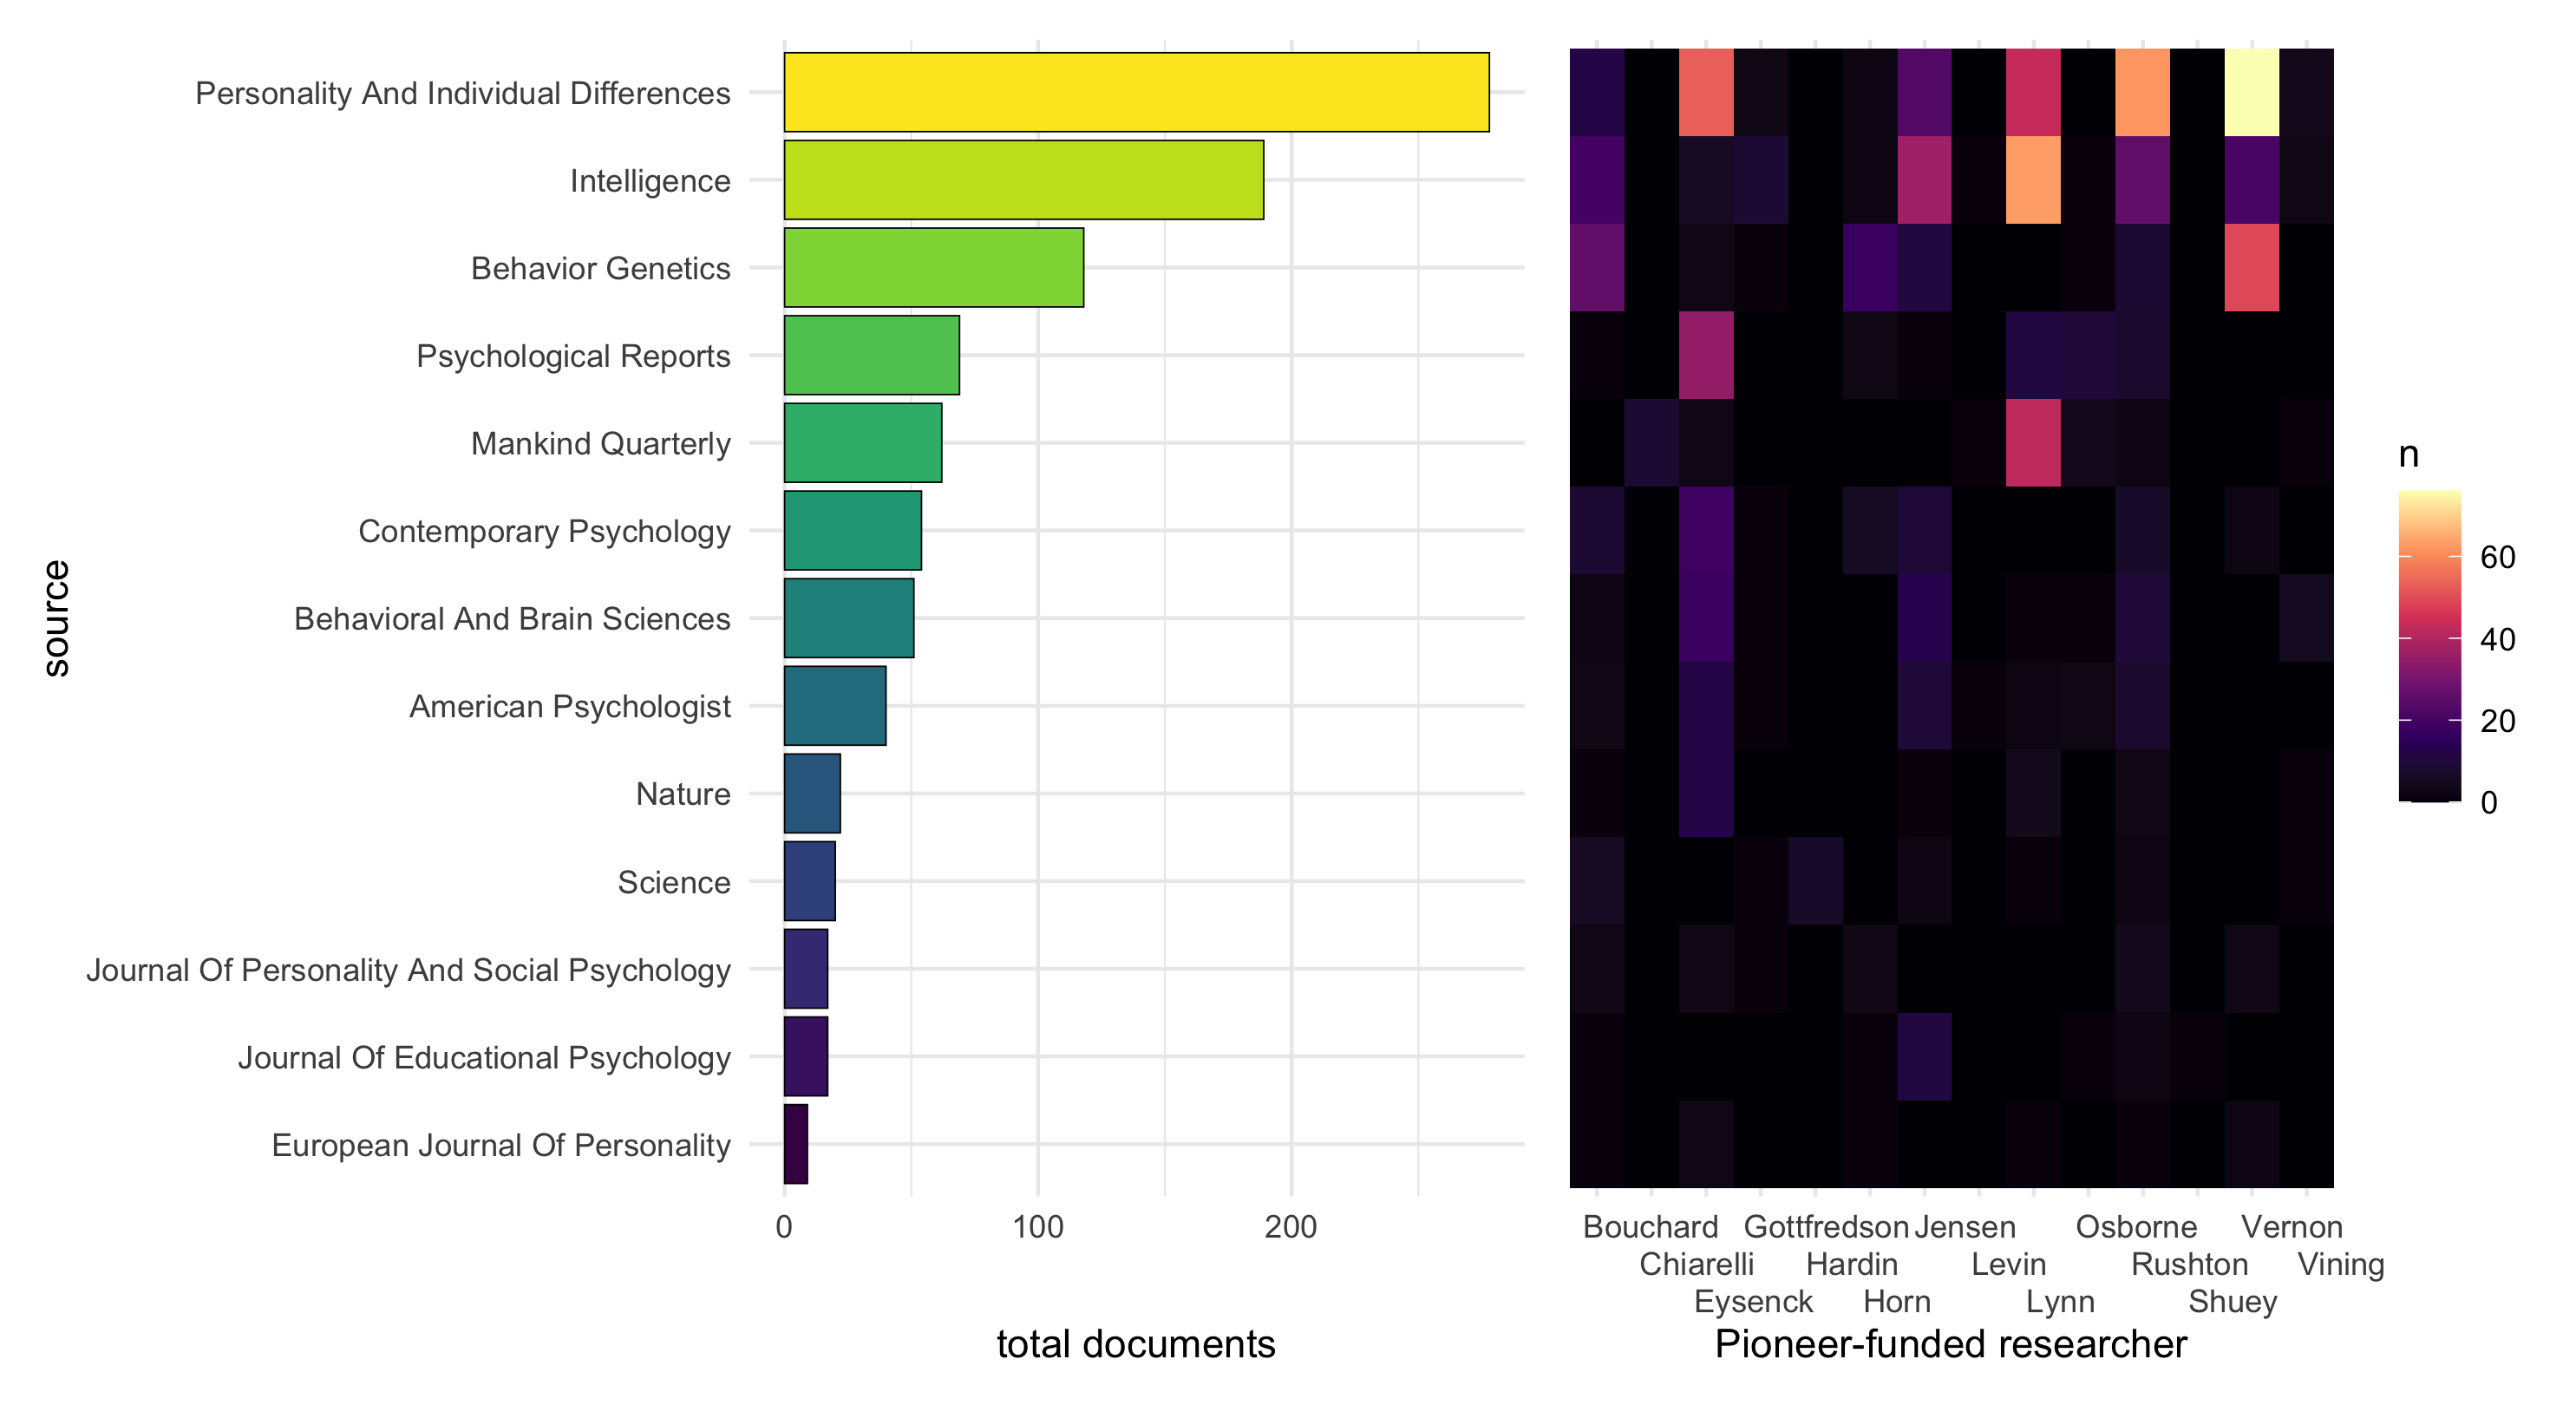
\includegraphics[width=4.76in,height=2.6in]{img/wos_results.png}
\caption{Journals publishing 6 or more Pioneer-funded researchers, WoS
author search results \emph{{[}date coverage{]}}}
\end{figure}

Figure \emph{{[}fig{]}} shows that, while MQ is on this list of
``Pioneer-publishing'' journals, a number of mainstream journals are
more prominent: \emph{Personality and Individual Differences} (PID),
\emph{Intelligence} (I), \emph{Behavior Genetics} (BG), and
\emph{Psychological Reports} (PR). In addition, only psychologist
Richard Lynn appears to have published heavily in MQ. Lynn has been an
assistant editor of MQ since 1979 \emph{{[}check this:
\url{https://rationalwiki.org/wiki/Mankind_Quarterly}{]}} and president
of PF since the death of psychologist J. Phillippe Rushton in 2012
\emph{{[}cite{]}}. By contrast, a number of Pioneer-funded researchers
have published in PID, I, and to a lesser degree BG: Eysenck, Jensen,
Rushton, Vernon, and also Lynn.

PID was founded in 1980, with Eysenck as editor-in-chief and an
editorial board including Jensen and Lynn. In the inaugural editorial,
Eysenck identified ``studies of the genetic determinants of individual
differences in the areas of personality and intelligence'' as one of the
journal's eight major areas of interest. Eysenck remained
editor-in-chief until his death in 1997. In 2005 the editorial board
still included Jensen and Lynn. PID was first published by Pergamon
Press, a mainstream academic press, and today is published by Elsevier.
According to the Scimago Journal Rankings, based on Scopus citation
data, in 2022 PID had an H-index of 193, \#29 in Psychology, and a
citation index of 5.27, \#24 in Psychology.

\emph{{[}similar para on I{]}}

\emph{{[}segue to topic model analysis{]}}

\hypertarget{topic-model-analysis}{%
\section*{Topic model analysis}\label{topic-model-analysis}}

\emph{{[}max \textasciitilde50 refs{]}}
\bibliography{references.bib}
\bibliographystyle{Science}

% Following is a new environment, {scilastnote}, that's defined in the
% preamble and that allows authors to add a reference at the end of the
% list that's not signaled in the text; such references are used in
% *Science* for acknowledgments of funding, help, etc.

\begin{scilastnote}
\item \emph{{[}strutured{]}} Thanks to Emily Merchant and John Jackson
for some initial discussions that helped clarify the scope of the
project and identify some key resources related to the Pioneer Fund and
\emph{Mankind Quarterly}. Thanks to Anthony Sainez for help retrieving
the \emph{Mankind Quarterly} articles. Thanks to Derek Devnich and James
Dooley for their work attempting to secure the APA-published articles.
EL's work on this project was supported by UC Merced. DH's work on this
project was not supported by any specific funding.
\end{scilastnote}


\renewcommand{\thetable}{\arabic{table}}
\renewcommand{\thefigure}{\arabic{figure}}
\setcounter{table}{0}
\setcounter{figure}{0}

%%%begfigs---

%%%endfigs---

%%%begtabs---

%%%endtabs---

% Needs a bit of work on the \ref{} TODO  before uncommenting
%\renewcommand{\thetable}{A\arabic{table}}
%\renewcommand{\thefigure}{A\arabic{figure}}
%\setcounter{table}{0}
%\setcounter{figure}{0}

%%%begappxfigs---

%%%endappxfigs---

%%%begappxtabs---

%%%endappxtabs---

\end{document}
